\documentclass[tikz]{standalone}

\usepackage{amsmath}
\usepackage{unicode-math}
\usepackage{mathtools}
\usepackage{derivative}

\setmainfont{Stix Two Text}
\setmathfont{Stix Two Math}

\usetikzlibrary{arrows.meta,fit,positioning}

\renewcommand{\familydefault}{\sfdefault}

% prefix equation numbers with section number
\numberwithin{equation}{section}

\DeclarePairedDelimiter{\ceil}{\lceil}{\rceil}
\DeclarePairedDelimiter{\floor}{\lfloor}{\rfloor}
\DeclarePairedDelimiter{\abs}{\lvert}{\rvert}
\DeclarePairedDelimiter{\norm}{\lVert}{\rVert}
\DeclarePairedDelimiter{\bra}{\langle}{\rvert}
\DeclarePairedDelimiter{\ket}{\lvert}{\rangle}
\DeclarePairedDelimiter{\expval}{\langle}{\rangle}
\DeclarePairedDelimiter{\norder}{\mathcolon}{\mathcolon}
\DeclarePairedDelimiter{\anorder}{\typecolon}{\typecolon}
	
\newcommand{\laplace}{\mbfnabla^2}
\newcommand{\trans}{{\scriptscriptstyle\mathsf{T}}}

\newcommand{\vdot}{\cdot}
\newcommand{\vcross}{\vectimes}
\newcommand{\vb}[1]{\symbfup{#1}}
\newcommand{\vu}[1]{\hat{\vb{#1}}}
\newcommand*\dd[2][\relax]{\mathop{\ifx\relax#1\odif{#2}\else \odif[order={#1}]{#2}\fi\,}}

\newcommand{\vacuum}{\ket*{\vb{0}}}

\DeclareMathOperator{\trace}{Tr}
\DeclareMathOperator{\sinc}{sinc}

\AtBeginDocument{
	\let\Re\relax
	\let\Im\relax
	\DeclareMathOperator{\Re}{Re}
	\DeclareMathOperator{\Im}{Im}

	\renewcommand{\div}{\mathop{\mbfnabla\vdot}}
	\newcommand{\curl}{\mathop{\mbfnabla\vectimes}}
}

\DeclarePairedDelimiterX{\comm}[2]{[}{]}{#1,#2}

\DeclarePairedDelimiterX{\braket}[2]{\langle}{\rangle}{#1\delimsize\vert#2}
\DeclarePairedDelimiterX{\ketbra}[1]{\lvert}{\rvert}{#1\rangle\delimsize\langle#1}



\begin{document}
	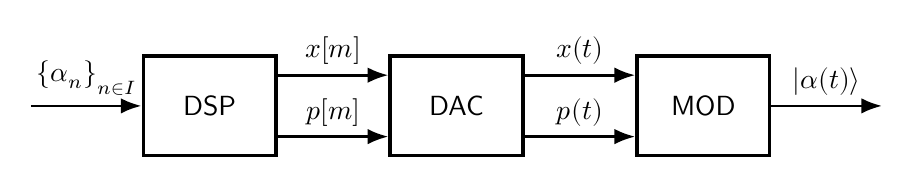
\begin{tikzpicture}[
		line width=1pt,
		node distance=40pt,
		block/.style={draw, very thick, fill=white, minimum height=36pt, minimum width=48pt},
		arrow/.style={-Latex},
	]
		\coordinate (in) at (0,0);
		\node (dsp) [block, right=of in] {DSP};
		\node (dac) [block, right=of dsp] {DAC};
%		\node (asp) [block, right=of dac] {ASP};
		\node (mod) [block, right=of dac] {MOD};
		\coordinate[right=of mod] (out);
		
		\draw[arrow] (in) -- (dsp) node[midway, above]{$\left\{\alpha_n\right\}_{n\in I}$};
		\draw[arrow] ([yshift=2.5ex]dsp.east) -- ([yshift=2.5ex]dac.west) node[midway, above]{$x[m]$};
		\draw[arrow] ([yshift=-2.5ex]dsp.east) -- ([yshift=-2.5ex]dac.west) node[midway, above]{$p[m]$};
	%	\draw[arrow] ([yshift=-2.5ex]dac.east) -- ([yshift=-2.5ex]asp.west) node[midway, above]{$p^\prime(t)$};
	%	\draw[arrow] ([yshift=2.5ex]dac.east) -- ([yshift=2.5ex]asp.west) node[midway, above]{$x^\prime(t)$};
		\draw[arrow] ([yshift=2.5ex]dac.east) -- ([yshift=2.5ex]mod.west) node[midway, above]{$x(t)$};
		\draw[arrow] ([yshift=-2.5ex]dac.east) -- ([yshift=-2.5ex]mod.west) node[midway, above]{$p(t)$};
		\draw[arrow] (mod) -- (out) node[midway, above]{$\ket{\alpha(t)}$};
		
		%\draw[drange] (in) ++(0,-1) coordinate (dom) -- ++(4.2,0) node[midway, below] {Digital};
		%\draw[drange] (dom-|dac.south) ++(0.1,0) -- ++(4.8,0) node[midway, below] {Analog};
		%\draw[drange] (dom-|mod.south) ++(0.15,0) -- (dom-|out) node[midway, below] {Quantum};
	\end{tikzpicture}
\end{document}
